% Options for packages loaded elsewhere
\PassOptionsToPackage{unicode}{hyperref}
\PassOptionsToPackage{hyphens}{url}
%
\documentclass[
  11pt,
  a4paper,
]{article}
\usepackage{amsmath,amssymb}
\usepackage{lmodern}
\usepackage{iftex}
\ifPDFTeX
  \usepackage[T1]{fontenc}
  \usepackage[utf8]{inputenc}
  \usepackage{textcomp} % provide euro and other symbols
\else % if luatex or xetex
  \ifXeTeX
    \usepackage{zxjatype} 
    \usepackage[ipaex]{zxjafont}
    \setromanfont{Times New Roman}
  \fi
  \usepackage{unicode-math}
  \defaultfontfeatures{Scale=MatchLowercase}
  \defaultfontfeatures[\rmfamily]{Ligatures=TeX,Scale=1}
\fi
% Use upquote if available, for straight quotes in verbatim environments
\IfFileExists{upquote.sty}{\usepackage{upquote}}{}
\IfFileExists{microtype.sty}{% use microtype if available
  \usepackage[]{microtype}
  \UseMicrotypeSet[protrusion]{basicmath} % disable protrusion for tt fonts
}{}
\usepackage{xcolor}
\IfFileExists{xurl.sty}{\usepackage{xurl}}{} % add URL line breaks if available
\IfFileExists{bookmark.sty}{\usepackage{bookmark}}{\usepackage{hyperref}}
\hypersetup{
  pdftitle={Appendix ``Text-Based Nudges Promoting Rubella Antibody Testing and Vaccination: Evidence from Nationwide Online Field Experiment in Japan''},
  hidelinks,
  pdfcreator={LaTeX via pandoc}}
\urlstyle{same} % disable monospaced font for URLs
\usepackage[left=3cm,right=3cm,top=3cm,bottom=3cm]{geometry}

\usepackage{setspace}
\renewcommand{\baselinestretch}{1.5}
\usepackage{float}

\usepackage{longtable,booktabs,array}
\usepackage{threeparttable, threeparttablex, multirow}
\usepackage{calc} % for calculating minipage widths
% Correct order of tables after \paragraph or \subparagraph
\usepackage{etoolbox}
\makeatletter
\patchcmd\longtable{\par}{\if@noskipsec\mbox{}\fi\par}{}{}
\makeatother
% Allow footnotes in longtable head/foot
\IfFileExists{footnotehyper.sty}{\usepackage{footnotehyper}}{\usepackage{footnote}}
\makesavenoteenv{longtable}
\usepackage{graphicx}
\makeatletter
\def\maxwidth{\ifdim\Gin@nat@width>\linewidth\linewidth\else\Gin@nat@width\fi}
\def\maxheight{\ifdim\Gin@nat@height>\textheight\textheight\else\Gin@nat@height\fi}
\makeatother
% Scale images if necessary, so that they will not overflow the page
% margins by default, and it is still possible to overwrite the defaults
% using explicit options in \includegraphics[width, height, ...]{}
\setkeys{Gin}{width=\maxwidth,height=\maxheight,keepaspectratio}
% Set default figure placement to htbp
\makeatletter
\def\fps@figure{htbp}
\makeatother
\setlength{\emergencystretch}{3em} % prevent overfull lines
\providecommand{\tightlist}{%
  \setlength{\itemsep}{0pt}\setlength{\parskip}{0pt}}
\setcounter{secnumdepth}{5}


\usepackage{float}
\ifLuaTeX
  \usepackage{selnolig}  % disable illegal ligatures
\fi

\makeatletter
\def\@fnsymbol#1{\ensuremath{\ifcase#1\or \dagger\or \ddagger\or
   \mathsection\or \mathparagraph\or \|\or **\or \dagger\dagger
   \or \ddagger\ddagger \else\@ctrerr\fi}}
    \makeatother
\title{Appendix
``Text-Based Nudges Promoting Rubella Antibody Testing and Vaccination:
Evidence from Nationwide Online Field Experiment in Japan''  }

\date{2022/04/15}



\begin{document}
\begin{spacing}{1}
  \maketitle
\end{spacing}

{
\setcounter{tocdepth}{2}
\tableofcontents
}
\hypertarget{appendix-appendix}{%
\appendix}


\hypertarget{overview-of-online-survey-experiment}{%
\section{Overview of Online Survey Experiment}\label{overview-of-online-survey-experiment}}

\begin{figure}[t]
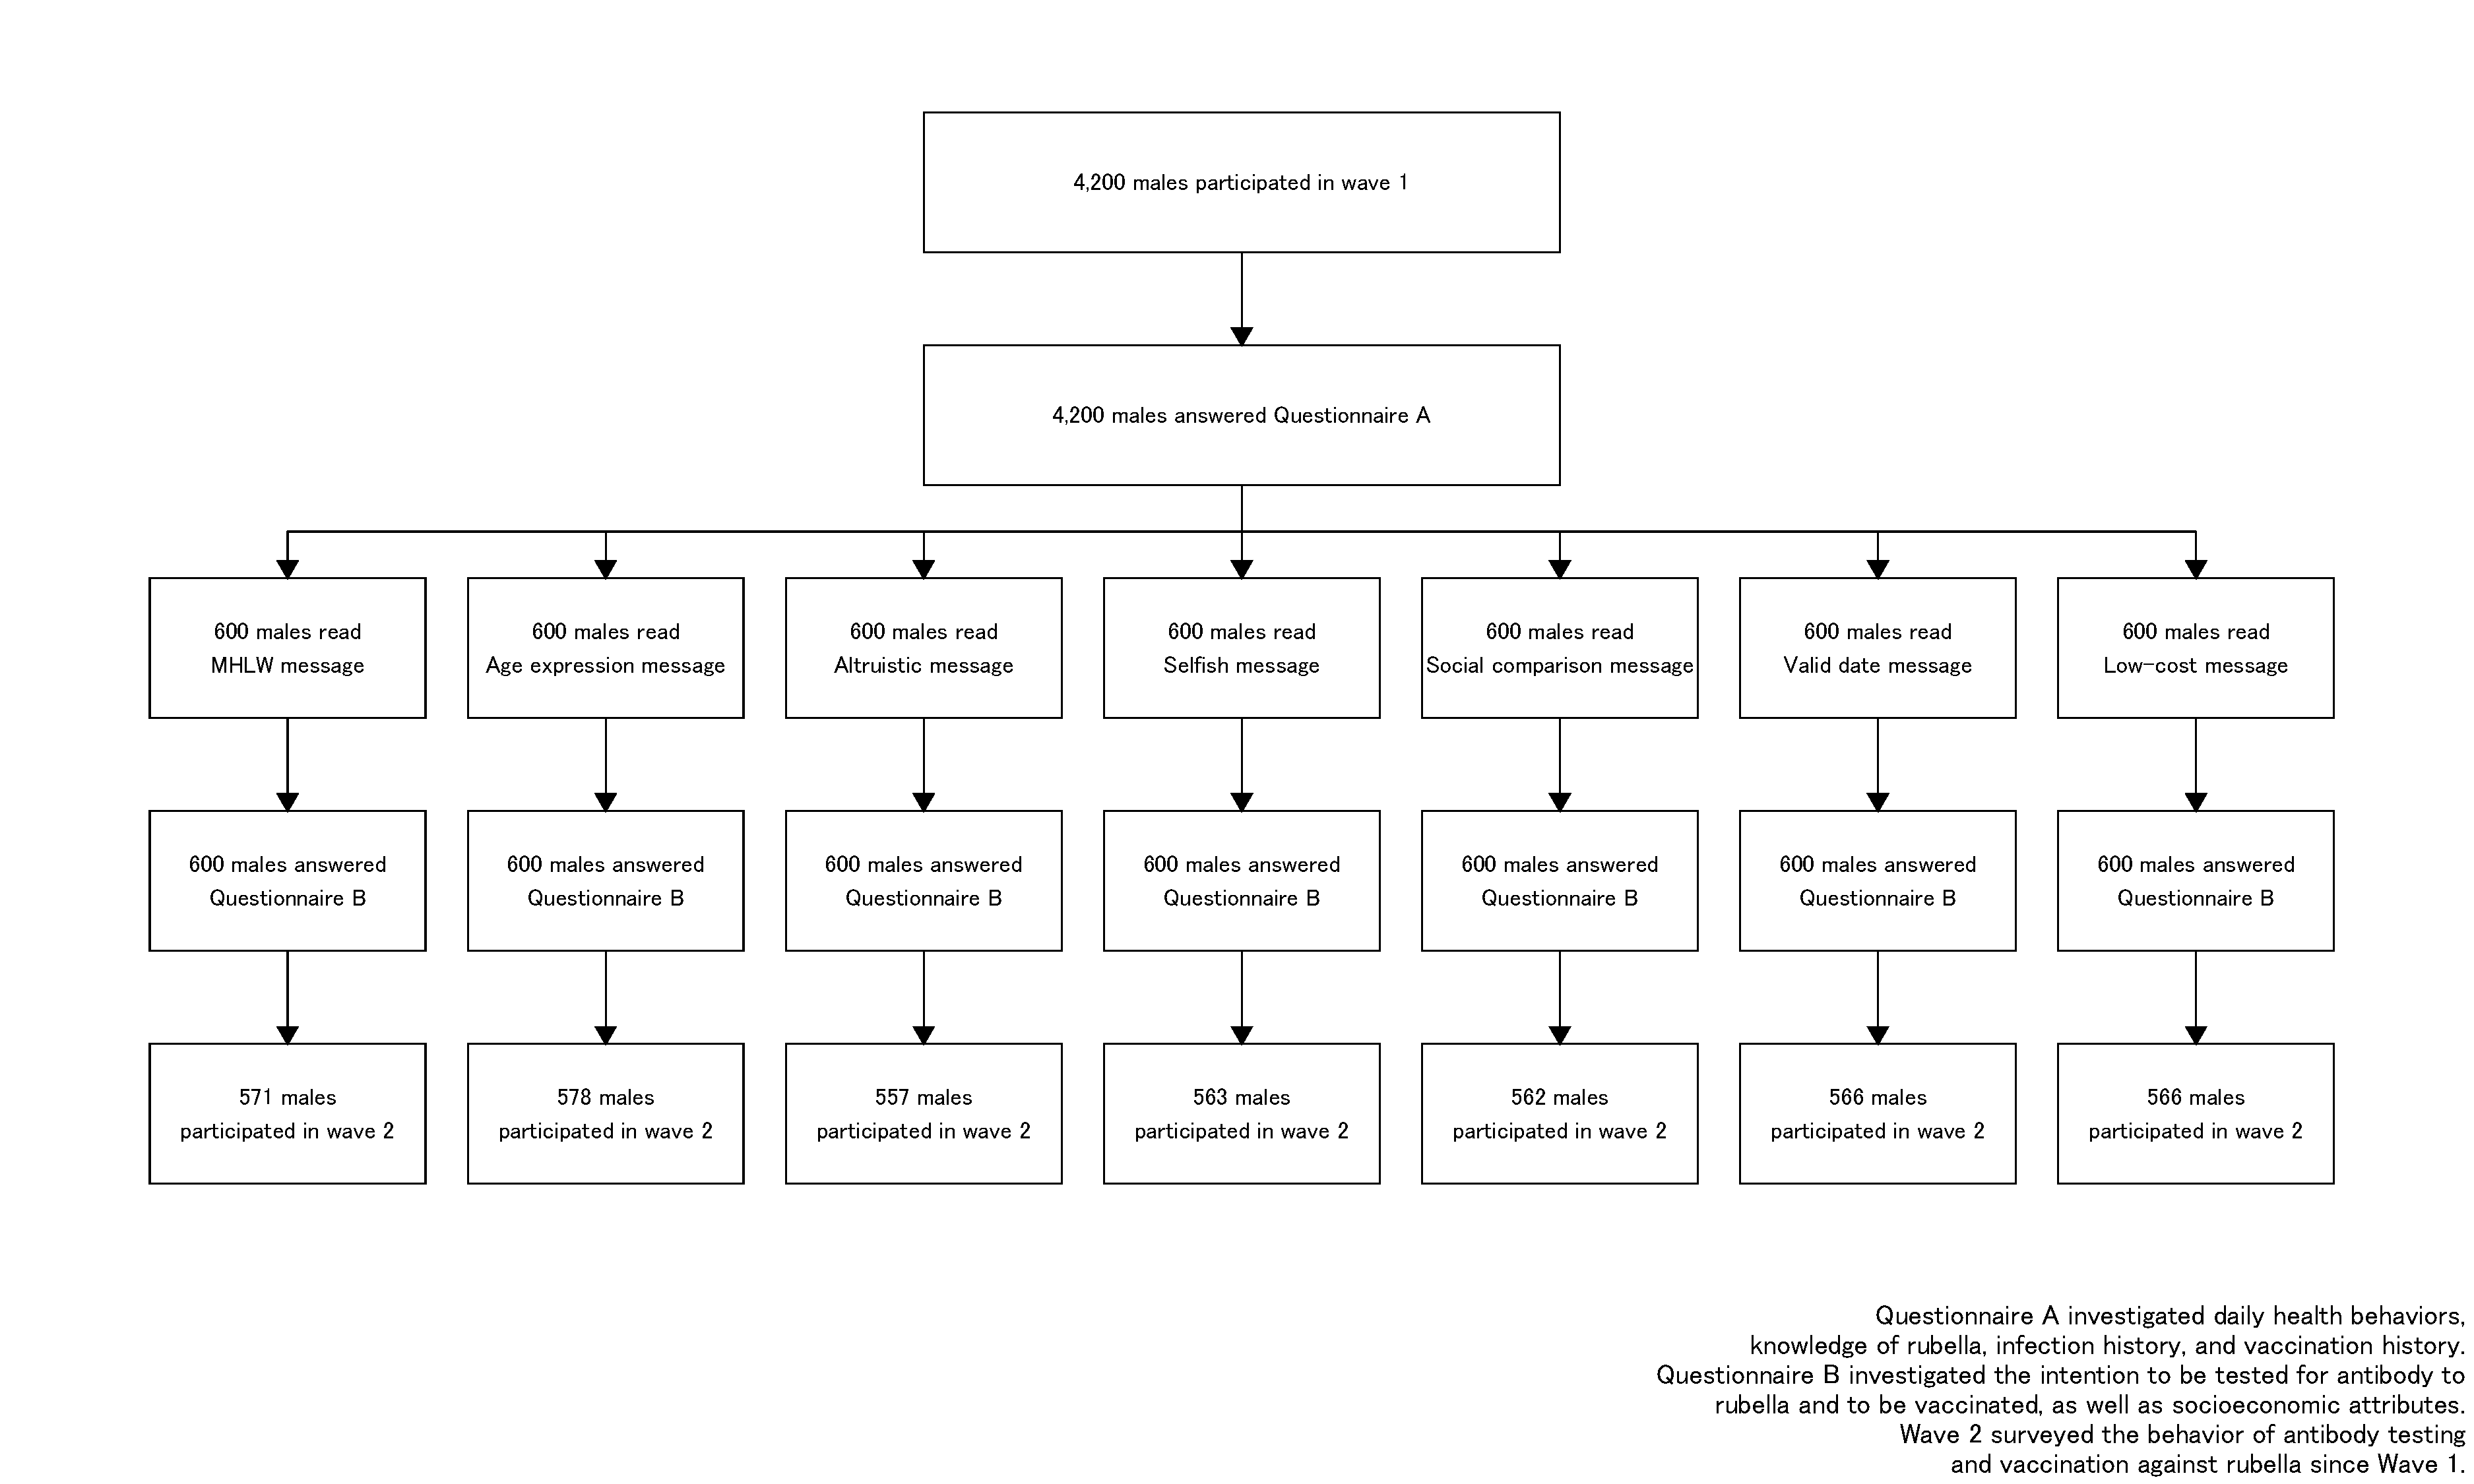
\includegraphics[width=1.5\linewidth,angle=90]{C:/Users/vge00/Desktop/2020-online-RCT/publish/appendix_files/figure-latex/flowchart-1} \caption{Overview of Online Survey Experiment}\label{fig:flowchart}
\end{figure}

\begin{table}[!h]

\caption{\label{tab:covlist}List of Covariates}
\centering
\fontsize{9}{11}\selectfont
\begin{tabular}[t]{l>{\raggedright\arraybackslash}p{30em}cc}
\toprule
  & Description & Mean & Std.Dev.\\
\midrule
age & (Wave1) Age as of April 2019 based on year of birth and month of birth. & 48.66 & 5.69\\
coupon2019 & (Wave1) Dummy variable taking one if 40 to 46 years old as of April 2019. & 0.35 & 0.48\\
married & (Wave1) Dummy variable taking one if a respondent is married. & 0.58 & 0.49\\
education & (Wave1) Years of education. & 14.75 & 2.31\\
exercise\_w1 & (Wave1) Dummy variable taking one if a respondent exercises or plays sports more than once a week. & 0.22 & 0.42\\
health\_check & (Wave1) Dummy variable taking one if a respondent has had medical examination at his/her city or place of employment in the past year from the time of the wave 1. & 0.68 & 0.46\\
flushot & (Wave1) Dummy variable taking one if a respondent is vaccinated against influenza every year. & 0.27 & 0.45\\
prob\_social & (Wave1) What percentage of men in their 40s and 50s does a respondent think may be infected with rubella? & 30.38 & 19.87\\
handicap & (Wave1) Dummy variable taking one if a respondent believes that if a woman in early pregnancy is infected with rubella, her child may be born with a disability. & 0.63 & 0.48\\
severity & (Wave1) Dummy variable taking one if a respondent believes that if an adult male is infected with rubella, it will become more severe. & 0.92 & 0.27\\
handwash & (Wave2) Five Likert scale for the question "I wash my hands and gargle frequently during the period from the end of the previous questionnaire response to today." & 3.91 & 1.04\\
temp\_check & (Wave2) Five Likert scale for the question "I take my tempature frequently during the period from the end of the previous questionnaire response to today." & 2.26 & 1.22\\
avoid\_out & (Wave2) Five Likert scale for the question "I am refraining from going out during the end of the previous questionnaire response to today." & 2.96 & 1.20\\
avoid\_crowd & (Wave2) Five Likert scale for the question "I avoid crowded places when I go out from the end of the previous questionnaire response to today." & 3.38 & 1.10\\
wear\_mask & (Wave2) Five Likert scale for the question "I always wear a medical mask when I go out or meet people during the period from the end of the previous questionnaire response to today." & 3.14 & 1.38\\
\bottomrule
\end{tabular}
\end{table}

\clearpage

\hypertarget{estimation-results-of-linear-probability-models}{%
\section{Estimation Results of Linear Probability Models}\label{estimation-results-of-linear-probability-models}}

\begin{table}

\caption{\label{tab:int-reg}Linear Probability Model of Intentions}
\centering
\begin{tabular}[t]{lcc}
\toprule
\multicolumn{1}{c}{ } & \multicolumn{1}{c}{Antibody Test} & \multicolumn{1}{c}{Vaccination} \\
\cmidrule(l{3pt}r{3pt}){2-2} \cmidrule(l{3pt}r{3pt}){3-3}
  & (1) & (2)\\
\midrule
Age expression & -0.036 & -0.099**\\
 & (0.038) & (0.043)\\
Altruistic & 0.051 & -0.059\\
 & (0.042) & (0.045)\\
Selfish & 0.026 & -0.052\\
 & (0.040) & \vphantom{1} (0.043)\\
Social comparison & -0.044 & -0.098**\\
 & (0.038) & (0.042)\\
Valid date & 0.028 & -0.044\\
 & (0.039) & (0.043)\\
Low-cost & 0.032 & -0.051\\
 & (0.040) & (0.043)\\
Coupon & -0.072 & -0.074\\
 & (0.052) & (0.062)\\
Coupon×Age expression & 0.045 & 0.103\\
 & (0.063) & (0.075)\\
Coupon×Altruistic & 0.089 & 0.073\\
 & (0.067) & (0.075)\\
Coupon×Selfish & 0.059 & 0.099\\
 & (0.066) & (0.075)\\
Coupon×Social comparison & 0.122* & 0.127*\\
 & (0.065) & \vphantom{1} (0.075)\\
Coupon×Valid date & -0.006 & 0.026\\
 & (0.064) & (0.074)\\
Coupon×Low-cost & 0.015 & 0.064\\
 & (0.065) & (0.075)\\
\midrule
Num.Obs. & 2459 & 2459\\
R2 & 0.363 & 0.530\\
R2 Adj. & 0.355 & 0.524\\
Covariates & X & X\\
\bottomrule
\end{tabular}
\end{table}
\begin{table}

\caption{\label{tab:int-reg-ftest}Effects of Text-Based Nudges on Intentions Using Linear Probability Model Estimates}
\centering
\begin{tabular}[t]{lrrrrrrrrrrrr}
\toprule
\multicolumn{1}{c}{ } & \multicolumn{6}{c}{Antibody Test} & \multicolumn{6}{c}{Vaccination} \\
\cmidrule(l{3pt}r{3pt}){2-7} \cmidrule(l{3pt}r{3pt}){8-13}
\multicolumn{1}{c}{ } & \multicolumn{3}{c}{w/o receiving coupon automatically} & \multicolumn{3}{c}{w/ receiving coupon automatically} & \multicolumn{3}{c}{w/o receiving coupon automatically} & \multicolumn{3}{c}{w/ receiving coupon automatically} \\
\cmidrule(l{3pt}r{3pt}){2-4} \cmidrule(l{3pt}r{3pt}){5-7} \cmidrule(l{3pt}r{3pt}){8-10} \cmidrule(l{3pt}r{3pt}){11-13}
nudge & estimate & std.error & p.value & estimate  & std.error  & p.value  & estimate   & std.error   & p.value   & estimate    & std.error    & p.value   \\
\midrule
Age expression & -0.036 & 0.038 & 0.336 & 0.008 & 0.051 & 0.869 & -0.099 & 0.043 & 0.021 & 0.004 & 0.061 & 0.945\\
Altruistic & 0.051 & 0.042 & 0.229 & 0.140 & 0.052 & 0.007 & -0.059 & 0.045 & 0.191 & 0.014 & 0.060 & 0.810\\
Selfish & 0.026 & 0.040 & 0.520 & 0.085 & 0.052 & 0.101 & -0.052 & 0.043 & 0.235 & 0.048 & 0.061 & 0.435\\
Social comparison & -0.044 & 0.038 & 0.247 & 0.078 & 0.052 & 0.134 & -0.098 & 0.042 & 0.020 & 0.029 & 0.062 & 0.641\\
Valid date & 0.028 & 0.039 & 0.482 & 0.022 & 0.050 & 0.662 & -0.044 & 0.043 & 0.308 & -0.018 & 0.061 & 0.769\\
Low-cost & 0.032 & 0.040 & 0.422 & 0.048 & 0.051 & 0.345 & -0.051 & 0.043 & 0.244 & 0.014 & 0.062 & 0.826\\
\bottomrule
\end{tabular}
\end{table}

クーポン券が自動的に送付されるかどうかは年齢で決まるので、
サブサンプルを用いたナッジ・メッセージの効果は
クーポン券が自動的に送付されるかどうかだけでなく、
二つのサブサンプルの年齢の違いの影響を受けている。
この問題を排除するために、意向の線形確率モデルを推定した。
説明変数はナッジ・メッセージのダミー変数、
ナッジ・メッセージのダミー変数とクーポン券が自動的に送付されることを示すダミー変数の交差項、
そして年齢を含んだ共変量である。
意向の線形確率モデルは上述の結果と同じ結果を得られた(詳細は補論を参照せよ)。

クーポン券が自動的に送付されるかどうかは年齢で決まるので、
サブサンプルを用いたナッジ・メッセージの効果は
クーポン券が自動的に送付されるかどうかだけでなく、
二つのサブサンプルの年齢の違いの影響を受けている。
この問題を排除するために、我々は以下のような意向の線形確率モデルを推定した。
\begin{align}
  Y_{ij} = \alpha + \sum_j \beta_j \text{Message}_j
           + \sum_j \gamma_j (\text{Message}_j \times \text{Coupon}_i)
           + \delta \text{Coupon}_i + \lambda X'_{ij} + \epsilon_{ij},
\end{align}
ここで、\(\text{Message}_j\)は厚労省メッセージ群をコントロールとした介入群ダミーであり、
\(\text{Coupon}_i\)はクーポン券の自動送付を受け取ったことを示すダミー変数である。
\(X\)は個人の共変量ベクトルであり、年齢を含む。

関心のあるパラメータは\(\beta_j\)と\(\gamma_j\)である。
クーポン券の自動送付の対象でない男性におけるナッジ・メッセージ\(j\)の効果は\(\hat{\beta}_j\)である。
一方で、クーポン券の自動送付の対象である男性におけるナッジ・メッセージ\(j\)の効果は
\(\hat{\beta}_j + \hat{\gamma}_j\)である。

表\ref{tab:int-reg}は線形確率モデルの結果である。また、
表\ref{tab:int-reg-ftest}は線形確率モデルの推定値を用いたナッジ・メッセージの効果である。
2019年度にクーポン券が自動的に送付される男性における
利他強調メッセージの抗体検査の意向に対する効果は14\%ポイントであり、
t検定の結果と一致する。
対して、2019年度にクーポン券を取得するために手続きが必要な男性における
利他強調メッセージの抗体検査の意向に対する効果は5.1\%ポイントであり、
統計的に非有意である。
表\ref{tab:int-reg}より、この二つの効果の差は統計的に非有意である。

また、2019年度にクーポン券が自動的に送付される男性における
社会比較メッセージのワクチン接種の意向に対する効果は2.9\%ポイントであり、
統計的に非有意である。
対して、2019年度にクーポン券を取得するために手続きが必要な男性における
社会比較メッセージのワクチン接種の意向に対する効果は-9.8\%ポイントであり、
t検定で推定された効果より若干大きくなった。
表\ref{tab:int-reg}より、この二つの効果の差は統計的に10\%水準で有意である。

さらに、2019年度にクーポン券を取得するために手続きが必要な男性における
年齢表現メッセージのワクチン接種の意向に対する効果は-9.9\%ポイントであり、
統計的に5\%水準で有意である。
t検定で推定された効果の規模は-6.6\%ポイントであり、
共変量の有無で効果の規模が大きく異なる。

\begin{table}

\caption{\label{tab:act-reg}Linear Probability Model of Behaviors}
\centering
\begin{tabular}[t]{lcc}
\toprule
\multicolumn{1}{c}{ } & \multicolumn{1}{c}{Antibody Test} & \multicolumn{1}{c}{Vaccination} \\
\cmidrule(l{3pt}r{3pt}){2-2} \cmidrule(l{3pt}r{3pt}){3-3}
  & (1) & (2)\\
\midrule
Age expression & 0.003 & 0.004\\
 & (0.008) & (0.005)\\
Altruistic & 0.016 & 0.005\\
 & (0.011) & (0.005)\\
Selfish & 0.008 & 0.005\\
 & (0.010) & (0.005)\\
Social comparison & 0.021* & -0.001\\
 & (0.012) & (0.001)\\
Valid date & 0.009 & 0.005\\
 & (0.009) & (0.005)\\
Low-cost & 0.005 & -0.001\\
 & (0.008) & (0.001)\\
Coupon & 0.017 & 0.001\\
 & (0.020) & (0.011)\\
Coupon×Age expression & 0.029 & 0.004\\
 & (0.029) & (0.015)\\
Coupon×Altruistic & 0.057* & 0.033\\
 & (0.034) & (0.022)\\
Coupon×Selfish & 0.054 & 0.014\\
 & (0.033) & (0.019)\\
Coupon×Social comparison & 0.036 & 0.041*\\
 & (0.035) & (0.023)\\
Coupon×Valid date & -0.002 & -0.005\\
 & (0.026) & (0.013)\\
Coupon×Low-cost & 0.033 & 0.020\\
 & (0.031) & (0.018)\\
\midrule
Num.Obs. & 2272 & 2272\\
R2 & 0.077 & 0.037\\
R2 Adj. & 0.066 & 0.025\\
Covariates & X & X\\
\bottomrule
\end{tabular}
\end{table}
\begin{table}

\caption{\label{tab:act-reg-ftest}Effects of Text-Based Nudges on Behaviors Using Linear Probability Model Estimates}
\centering
\begin{tabular}[t]{lrrrrrrrrrrrr}
\toprule
\multicolumn{1}{c}{ } & \multicolumn{6}{c}{Antibody Test} & \multicolumn{6}{c}{Vaccination} \\
\cmidrule(l{3pt}r{3pt}){2-7} \cmidrule(l{3pt}r{3pt}){8-13}
\multicolumn{1}{c}{ } & \multicolumn{3}{c}{w/o receiving coupon automatically} & \multicolumn{3}{c}{w/ receiving coupon automatically} & \multicolumn{3}{c}{w/o receiving coupon automatically} & \multicolumn{3}{c}{w/ receiving coupon automatically} \\
\cmidrule(l{3pt}r{3pt}){2-4} \cmidrule(l{3pt}r{3pt}){5-7} \cmidrule(l{3pt}r{3pt}){8-10} \cmidrule(l{3pt}r{3pt}){11-13}
nudge & estimate & std.error & p.value & estimate  & std.error  & p.value  & estimate   & std.error   & p.value   & estimate    & std.error    & p.value   \\
\midrule
Age expression & 0.003 & 0.008 & 0.724 & 0.032 & 0.028 & 0.259 & 0.004 & 0.005 & 0.413 & 0.008 & 0.014 & 0.592\\
Altruistic & 0.016 & 0.011 & 0.152 & 0.073 & 0.032 & 0.023 & 0.005 & 0.005 & 0.405 & 0.038 & 0.021 & 0.071\\
Selfish & 0.008 & 0.010 & 0.448 & 0.061 & 0.032 & 0.054 & 0.005 & 0.005 & 0.324 & 0.019 & 0.017 & 0.267\\
Social comparison & 0.021 & 0.012 & 0.084 & 0.057 & 0.032 & 0.077 & -0.001 & 0.001 & 0.538 & 0.040 & 0.023 & 0.078\\
Valid date & 0.009 & 0.009 & 0.339 & 0.007 & 0.025 & 0.775 & 0.005 & 0.005 & 0.317 & 0.000 & 0.012 & 0.991\\
Low-cost & 0.005 & 0.008 & 0.520 & 0.038 & 0.029 & 0.193 & -0.001 & 0.001 & 0.610 & 0.019 & 0.018 & 0.279\\
\bottomrule
\end{tabular}
\end{table}

サブサンプルで推定されたナッジ・メッセージの効果は
クーポン券が自動的に送付されるかどうかだけでなく、
年齢の違いの影響を受けるので、
我々はこの問題を排除するために線形確率モデルを推定した。
行動の線形確率モデルは上述の結果と同じ結果を得られた。
それに加えて、2019年度にクーポン券が自動的に送付される男性において、
社会比較メッセージの抗体検査の受検率は厚労省メッセージよりも5.7\%ポイント高く、
これは統計的に10\%水準で有意である。

意向の線形確率モデルと同じように、我々は行動を被説明変数とした線形確率モデルを推定した。
表\ref{tab:act-reg}は線形確率モデルの結果である。また、
表\ref{tab:act-reg-ftest}は線形確率モデルの推定値を用いたナッジ・メッセージの効果である。

利他強調メッセージの効果に関する結果を概観する。
2019年度にクーポン券が自動的に送付される男性における
利他強調メッセージの抗体検査の受検率に対する効果は3.2\%ポイントであり、
t検定の結果と一致する。
対して、2019年度にクーポン券を取得するために手続きが必要な男性における
利他強調メッセージの抗体検査の受検率に対する効果は1.6\%ポイントであり、
統計的に非有意である。
表\ref{tab:act-reg}より、この二つの効果の差は統計的に10\%水準で有意である。
また、2019年度にクーポン券が自動的に送付される男性における
利他強調メッセージのワクチン接種率に対する効果は3.8\%ポイントであり、
t検定の結果と一致する。
対して、2019年度にクーポン券を取得するために手続きが必要な男性における
利他強調メッセージのワクチン接種率に対する効果は0.5\%ポイントであり、
統計的に非有意である。
表\ref{tab:act-reg}より、この二つの効果の差は統計的に非有意である。

次に、利己強調メッセージの効果に関する結果を概観する。
2019年度にクーポン券が自動的に送付される男性における
利己強調メッセージの抗体検査の受検率に対する効果は6.1\%ポイントであり、
t検定で推定された効果より大きくなる。
対して、2019年度にクーポン券を取得するために手続きが必要な男性における
利己強調メッセージの抗体検査の受検率に対する効果は0.8\%ポイントであり、
統計的に非有意である。
表\ref{tab:act-reg}より、この二つの効果の差は統計的に非有意である。
また、2019年度にクーポン券が自動的に送付される男性における
利己強調メッセージのワクチン接種率に対する効果は1.9\%ポイントであり、
統計的に非有意である。
対して、2019年度にクーポン券を取得するために手続きが必要な男性における
利己強調メッセージのワクチン接種率に対する効果は0.5\%ポイントであり、
統計的に非有意である。
表\ref{tab:act-reg}より、この二つの効果の差は統計的に非有意である。

最後に、社会比較メッセージの効果に関する結果を概観する。
2019年度にクーポン券が自動的に送付される男性における
社会比較メッセージの抗体検査の受検率に対する効果は5.7\%ポイントであり、
t検定で推定された効果と似ていて、統計的に10\%水準で有意である。
対して、2019年度にクーポン券を取得するために手続きが必要な男性における
利己強調メッセージの抗体検査の受検率に対する効果は2.1\%ポイントであり、
t検定の結果と近似している。
表\ref{tab:act-reg}より、この二つの効果の差は統計的に非有意である。
また、2019年度にクーポン券が自動的に送付される男性における
社会比較メッセージのワクチン接種率に対する効果は4\%ポイントであり、
t検定の結果と一致する。
対して、2019年度にクーポン券を取得するために手続きが必要な男性における
社会比較メッセージのワクチン接種率に対する効果は-0.1\%ポイントであり、
統計的に非有意である。
表\ref{tab:act-reg}より、この二つの効果の差は統計的に10\%水準で有意である。

\clearpage

\end{document}
